\documentclass[a4paper,10pt,oneside]{article}
\usepackage[polutonikogreek,italian]{babel}
\usepackage[utf8x]{inputenc}
\usepackage{amsmath}
\usepackage{amsthm}
\usepackage{amssymb}
\usepackage{amscd}
\usepackage{graphicx}
\usepackage{float}
\usepackage{array}
\usepackage{verbatim}
\usepackage{rotating}
\usepackage[small]{caption}
\usepackage{lscape}
\usepackage{fancybox}
\usepackage{booktabs}
\parindent0ex 
\renewcommand{\fboxsep}{0.5cm}
\usepackage{hyperref}
\renewcommand{\textfraction}{0.05}
\renewcommand{\topfraction}{0.95}
\renewcommand{\bottomfraction}{0.95}
\renewcommand{\floatpagefraction}{0.35}
\setcounter{totalnumber}{5}
\restylefloat{figure}
\newlength{\drop}
\begin{document}

\begin{center}
{\huge Laboratorio di calorimetria e termodinamica}
\end{center} 

\section{Calore ed attrito}

In questo esperimento misureremo il trasferimento di energia tramite lo sfregamento di uno spago su un cilindretto metallico. Facendo riferimento alla figura [\ref{fig:attrito1}]
\begin{figure}[H]
 \centering
 \includegraphics[width=\textwidth]{Immagini/attrito.png}
 % attrito.png: 1739x1168 pixel, 201dpi, 21.99x14.77 cm, bb=
 \caption{La forza di attrito $F_A$ ha sempre verso opposto allo spostamento il lavoro in un ciclo della forza d'attrito è quindi diverso da zero}
 \label{fig:attrito1}
\end{figure}
immaginiamo un processo quasi statico, ovvero un processo ove la velocità con cui la massa sospesa si muove è infinitesima ed un ciclo di sollevamento-abbassamento alla fine del quale la massa torna alla posizione di partenza.
Possiamo scrivere il lavoro della forza traente durante il processo sollevamento come:
\begin{equation}
 L_S=F_{TS}h
\end{equation}
 dove $h$ è la quota massima della massa sollevata e la forza di sollevamento $F_{TS}$ è in ogni istante:
\begin{equation}
 F_{TS}=mg+F_A
\end{equation}
dove $F_A$ è la forza di attrito esercitata nel punto di contatto dello spago con il cilindretto metallico.
Il lavoro fatto dalla forza traente durante il processo di abbassamento della massa sarà invece:
\begin{equation}
 L_{TA}=-F_{TA}h
\end{equation}
il segno negativo è dovuto al fatto che lo spostamento e la forza hanno versi opposti. La forza $F_{TA}$ è in questo caso (considerando il processo come quasi statico):
\begin{equation}
F_{TA}=mg-F_A
\end{equation}
Il lavoro totale fatto dalla forza traente nell'intero ciclo sarà quindi:

\begin{equation}
 L_{TS}+L_{TA}=(mg+F_A)h-(mg-F_A)h=2hF_A
\end{equation}
Le valutazioni precedenti valgono anche nel caso di processi non quasi statici, in tali casi è necessario utilizzare il calcolo differenziale per determinare il lavoro totale fatto dalla forza traente sul sistema. Dai calcoli precedenti possiamo vedere come il lavoro prodotto dalla forza $F_T$ sia uguale al lavoro della forza di attrito lungo tutto il percorso di lunghezza $2h$.
Se immaginiamo che tutto il lavoro dissipativo dell'attrito si trasformi in calore allora la variazione di entalpia del sistema sarà equivalente al calore fornito a pressione costante:
\begin{equation}\label{eq:en_int}
 \Delta H=Mc_P\Delta T= L_{TS}+L_{TA}
\end{equation}
dove $M$ è la massa del cilindretto $c_P$ il calore specifico e $T$ la variazione di temperatura assoluta. La variazione di energia interna del cilindretto metallico sarà quindi per il primo principio della termodinamica:
\begin{equation}
 \Delta U=L_{TS}+L_{TA} -p\Delta V
\end{equation}
siccome il lavoro svolto dal sistema a causa della variazione di volume del metallo sarà piccolo possiamo trascurare il termine $p\Delta V$ e ritenere l'aumento di energia interna del metallo equivalente al calore fornito al sistema tramite l'attrito dello spago con il cilindretto. 
\begin{equation}
 \Delta U= L_{TS}+L_{TA}
\end{equation}
da cui
\begin{equation}
 L_{TS}+L_{TA}=Mc_P\Delta T
\end{equation}

Nella realtà è impossibile riuscire a realizzare una trasformazione quasi statica, pertanto in laboratorio dovremmo effettuare un'analisi più complessa del processo di dissipazione del lavoro.
Introduciamo la potenza media $p_m$ definita come:
\begin{equation}
 p_m=\frac{\Delta L}{\Delta t}=\mathbf{F}_m\cdot \frac{\Delta \mathbf{s}}{\Delta t}=\mathbf{F}_m\cdot\mathbf{v}_m
\end{equation}
e la potenza istantanea:
\begin{equation}
 p=\frac{dL}{dt}=\mathbf{F}\cdot\frac{d\mathbf{s}}{dt}=\mathbf{F}\cdot\mathbf{v}
\end{equation}
dalle due relazioni precedenti vediamo come la potenza sia il prodotto scalare della forza e della velocità, ricordando la definizione di lavoro:
\begin{equation}
 L_{A\to B}=\int_A^B\mathbf{F}\cdot d\mathbf{s}
\end{equation}
e considerando il sistema nella posizione $A$ nell'istante $t_0$ e nella posizione $B$ nell'istante $t_1$ possiamo scrivere il lavoro come:
\begin{equation}\label{lav1}
 L_{A\to B}=\int_{t_0}^{t_1}\mathbf{F}\cdot\mathbf{v}dt
\end{equation}
Dalla relazione [\ref{lav1}] possiamo ricavare le grandezze da misurare in laboratorio: forza e velocità. Tramite un processo di integrazione numerica che verrà svolto dal software di acquisizione dati\footnote{Nulla vi vieta di effettuare l'integrazione con altri strumenti software} potremo quindi calcolare il lavoro svolto sul sistema (il cilindretto). Parallelamente all'acquisizione di forza e velocità misureremo anche la temperatura del cilindretto per confrontare il risultato teorico con l'aumento osservato. Nella relazione di laboratorio dovrete spiegare i motivi per cui l'innalzamento di temperatura è strettamente inferiore a quello previsto teoricamente \footnote{Il nostro semplice modello di trasferimento energetico non è quindi completo}.

\section{Misura del calore specifico}
In questo esperimento misureremo il calore specifico di varie sostanze presenti in laboratorio (rame, alluminio, ottone e tungsteno). La variazione di entalpia di un corpo a pressione costante è:
\begin{equation}
 \Delta H=M c_P\Delta T
\end{equation}
che corrisponde al calore scambiato con l'ambiente circostante a pressione costante.
Nel caso di un calorimetro perfetto, e con evaporazione minima, la variazione di entalpia dell'acqua deve essere uguale ed opposta a quella del metallo:
\begin{equation}\label{calo1}
 M_mc_m|\Delta T_m|=M_ac_a|\Delta T_a|
\end{equation}
dalla conoscenza del calore specifico dell'acqua $c_a=4186 JKg^{-1}K^{-1}$ possiamo dedurre il calore specifico del metallo immerso\footnote{Il calore specifico così calcolato sarà una stima abbastanza grossolana dato che non abbiamo considerato nella [\ref{calo1}] la variazione di entalpia del calorimetro}. Nota: in generale il calore specifico dipende dalla temperatura e può essere considerato costante solo per brevi intervalli di $T$ lontano dalle transizioni di fase.
\section{Calori latenti di liquefazione e vaporizzazione}

\subsection{Calore latente di vaporizzazione}
Quando il vapore entra in contatto con l'acqua fredda presente all'interno del calorimetro esso condensa e libera il calore latente di vaporizzazione, questa transizione di fase avviene ad una temperatura costante (100°C al livello del mare), quando il vapore si è trasformato in acqua si raffredda normalmente fino ad arrivare all'equilibrio termico con l'acqua presente nel calorimetro.
Ignorando la capacità termica del calorimetro (ed immaginando che questo sia perfettamente isolato dall'ambiente esterno) possiamo scrivere:
\begin{equation}
 M_vH_v+M_vc_a|\Delta T_v|=M_ac_a|\Delta T_a|
\end{equation}
dove $H_v$ è il calore latente di vaporizzazione.
Nota: prestate attenzione ai segni delle variazioni di temperatura
\subsection{Calore latente di liquefazione}

Se nel caso del vapore avevamo una cessione di calore all'acqua durante il processo di liquefazione in questo caso avremo una cessione di calore dall'acqua al ghiaccio in fase di scioglimento. Quando inseriamo del ghiaccio all'interno del calorimetro contenente dell'acqua ad una temperatura $T_i$ il ghiaccio deve assorbire energia dall'acqua per effettuare una transizione di fase dallo stato solido a quello liquido, soltanto quando tutto il ghiaccio si è sciolto l'acqua presente inizialmente nel calorimetro e il ghiaccio disciolto possono raggiungere l'equilibrio termico.
\begin{equation}
 M_gH_f+M_gc_a|\Delta T_g|=M_ac_a|\Delta T_a|
\end{equation}
$H_f$ è il calore latente di fusione del ghiaccio d'acqua.
Nota: prestate attenzione ai segni delle variazioni di temperatura
\section{Verifica della legge di Boyle}

La legge di Boyle afferma che a temperatura costante
\begin{equation}
 PV=k
\end{equation}
ovvero che il prodotto della pressione e del volume di un gas è costante. In laboratorio cercheremo di verificare questa legge utilizzando un sensore di pressione ed una siringa graduata. Il procedimento sperimentale è molto semplice:
\begin{itemize}
 \item Colleghiamo il sensore di pressione alla siringa e spostiamo lo stantuffo fino a che il volume del gas contenuto all'interno sia un certo $V_0$, lasciamo per qualche istante che la temperatura del gas espanso si equilibri e misuriamo la pressione
\item Ripetiamo il passo precedente fino ad esaurire la siringa
\end{itemize}

\section{Verifica della legge di Charles}

La legge di Charles nota anche come prima legge di Gay Lussac o di Volta-Gay Lussac ci dice che il volume di un gas aumenta linearmente con la temperatura:
\begin{equation}
 V(T_100)-V(T_0)=kV(T_0)
\end{equation}
utilizzando la legge dei gas perfetti possiamo scrivere:
\begin{equation}
 V(T_100)-V(T_0)=\Delta T\frac{NR}{P}
\end{equation}
quindi:
\begin{equation}
\frac{\Delta V_{100}}{V(T_0)}=\frac{\Delta T}{T_0}=\frac{100}{T_0}
\end{equation}
in laboratorio misureremo il volume di una certa quantità di gas alla temperatura di $0C°$ e mantenendo la pressione costante quello della stessa quantità di gas alla temperatura di $100C°$ da queste misurazioni dedurremo il valore della costante $k$ e quindi la temperatura assoluta del punto di congelamento dell'acqua.






\end{document}
